\documentclass{standalone}

\usepackage{tikz}
\usetikzlibrary{patterns,arrows,calc,decorations.pathmorphing,backgrounds, positioning,fit,petri,decorations.fractals,trees, matrix}
\usepackage{amsfonts}

\begin{document}
	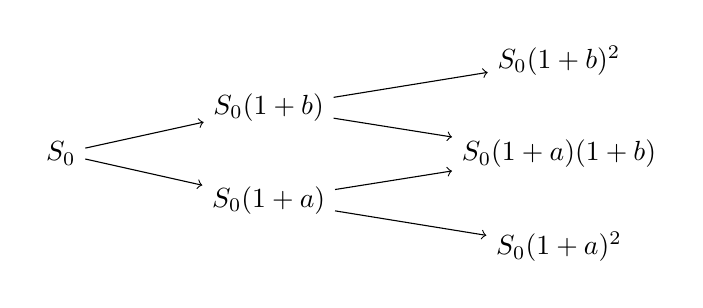
\begin{tikzpicture}
		\matrix (tree) [matrix of nodes,column sep=1.5cm]
		{
			      &              & $S_0 (1+b)^2$    \\
			      & $S_0 (1+b)$  &                  \\
			$S_0$ &              & $S_0 (1+a)(1+b)$ \\
			      & $S_0 (1+a)$  &                  \\
				  &              & $S_0 (1+a)^2$    \\
		};
		\draw[->] (tree-3-1)--(tree-2-2);
		\draw[->] (tree-3-1)--(tree-4-2);
		%%
		\draw[->] (tree-2-2)--(tree-1-3);
		\draw[->] (tree-2-2)--(tree-3-3);
		\draw[->] (tree-4-2)--(tree-3-3);
		\draw[->] (tree-4-2)--(tree-5-3);
	\end{tikzpicture}

\end{document}